\begin{figure}[!t]
    \centering
    % 
\includegraphics[width=0.6\columnwidth]{figures/overview/live_evaluation_over_time.png}
    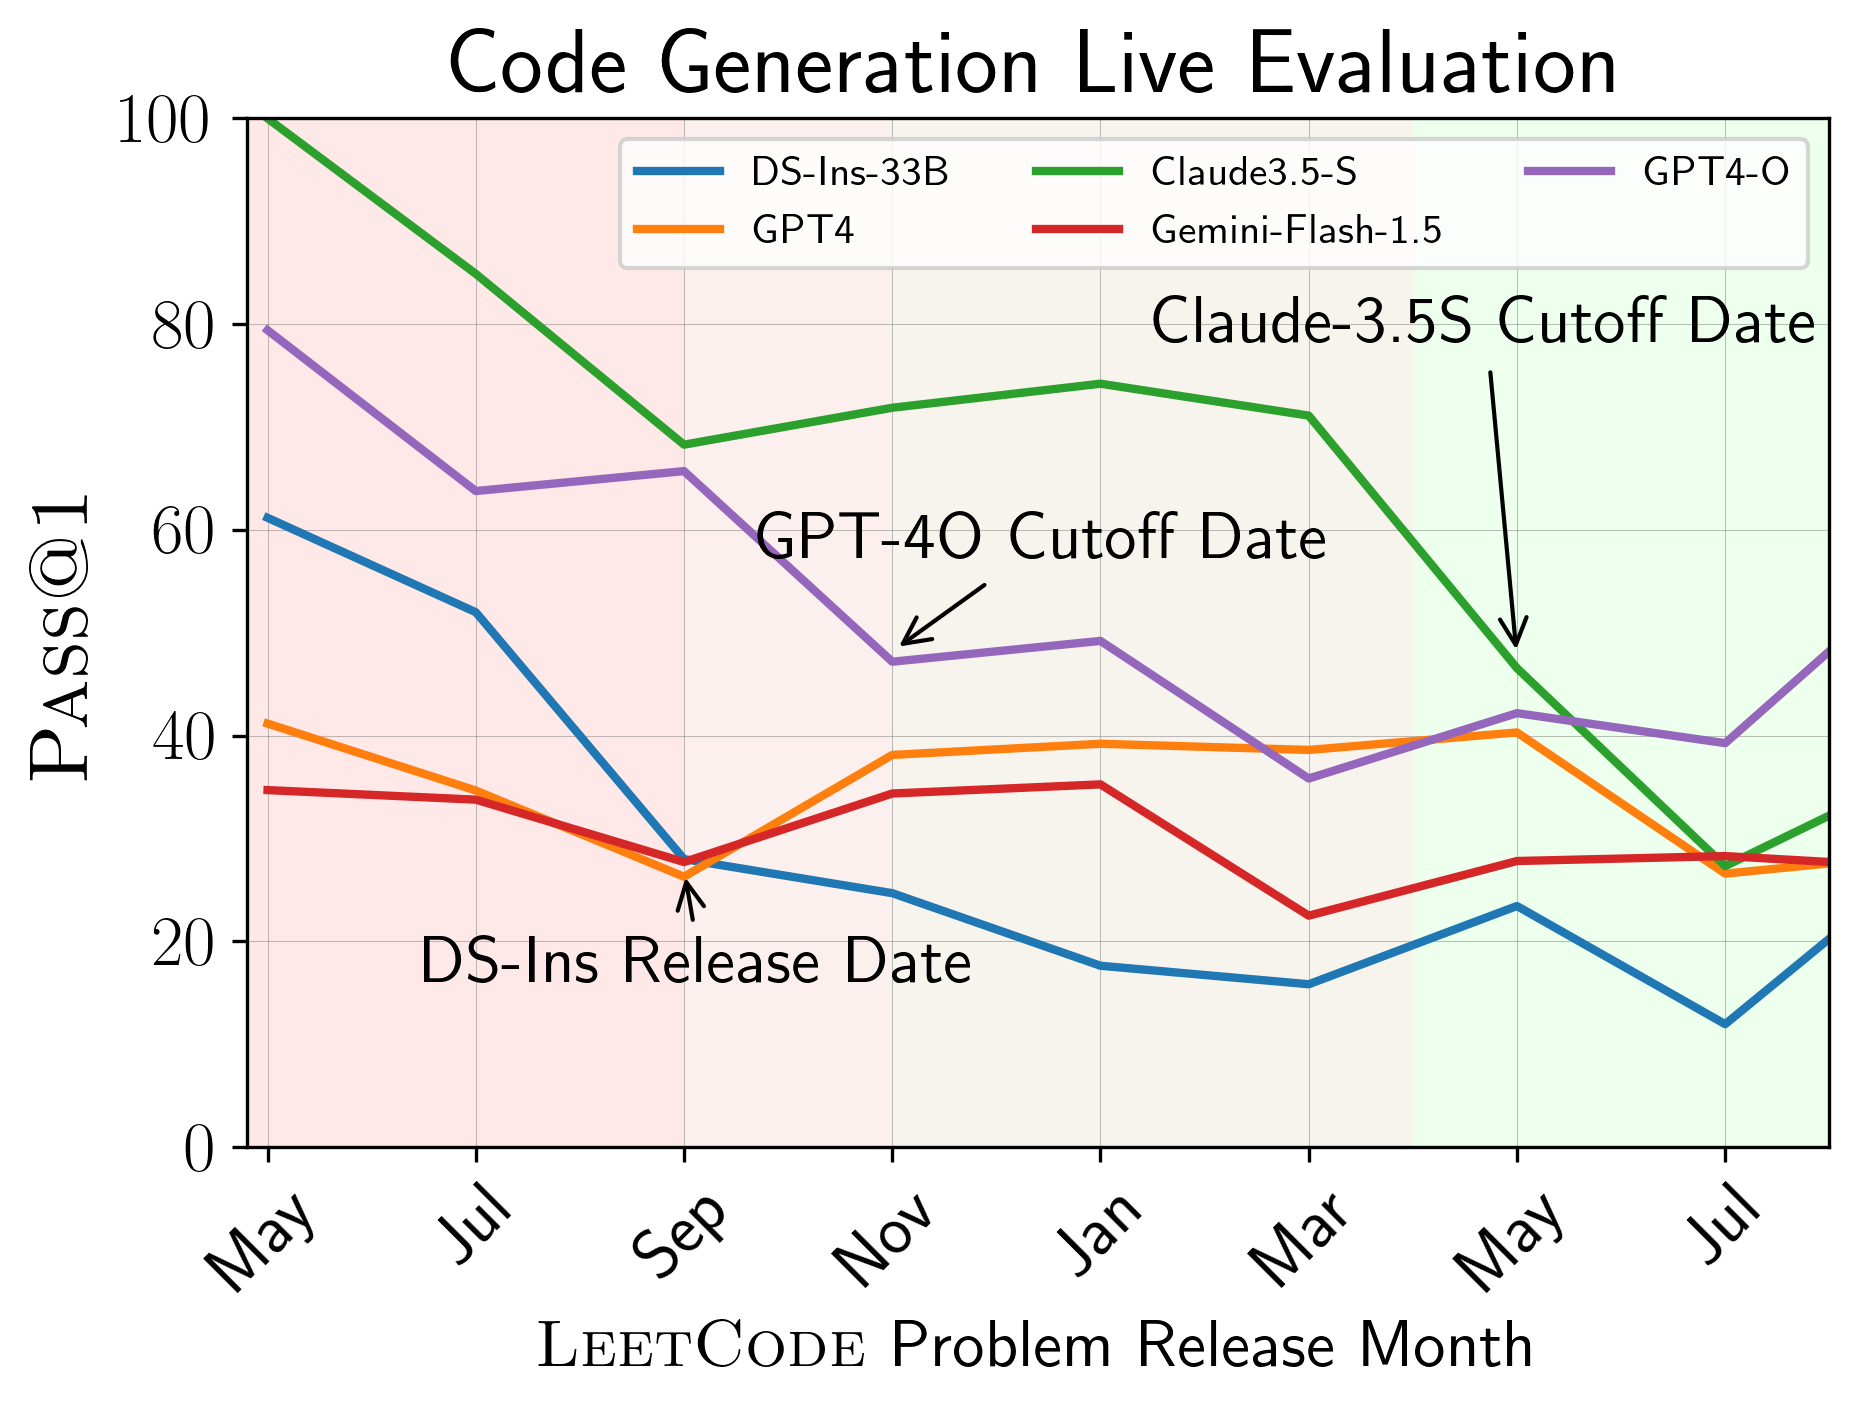
\includegraphics[width=0.50\linewidth]{figures/contamination_new/main_20_codegen_leetcode.png}
    \hfil%
        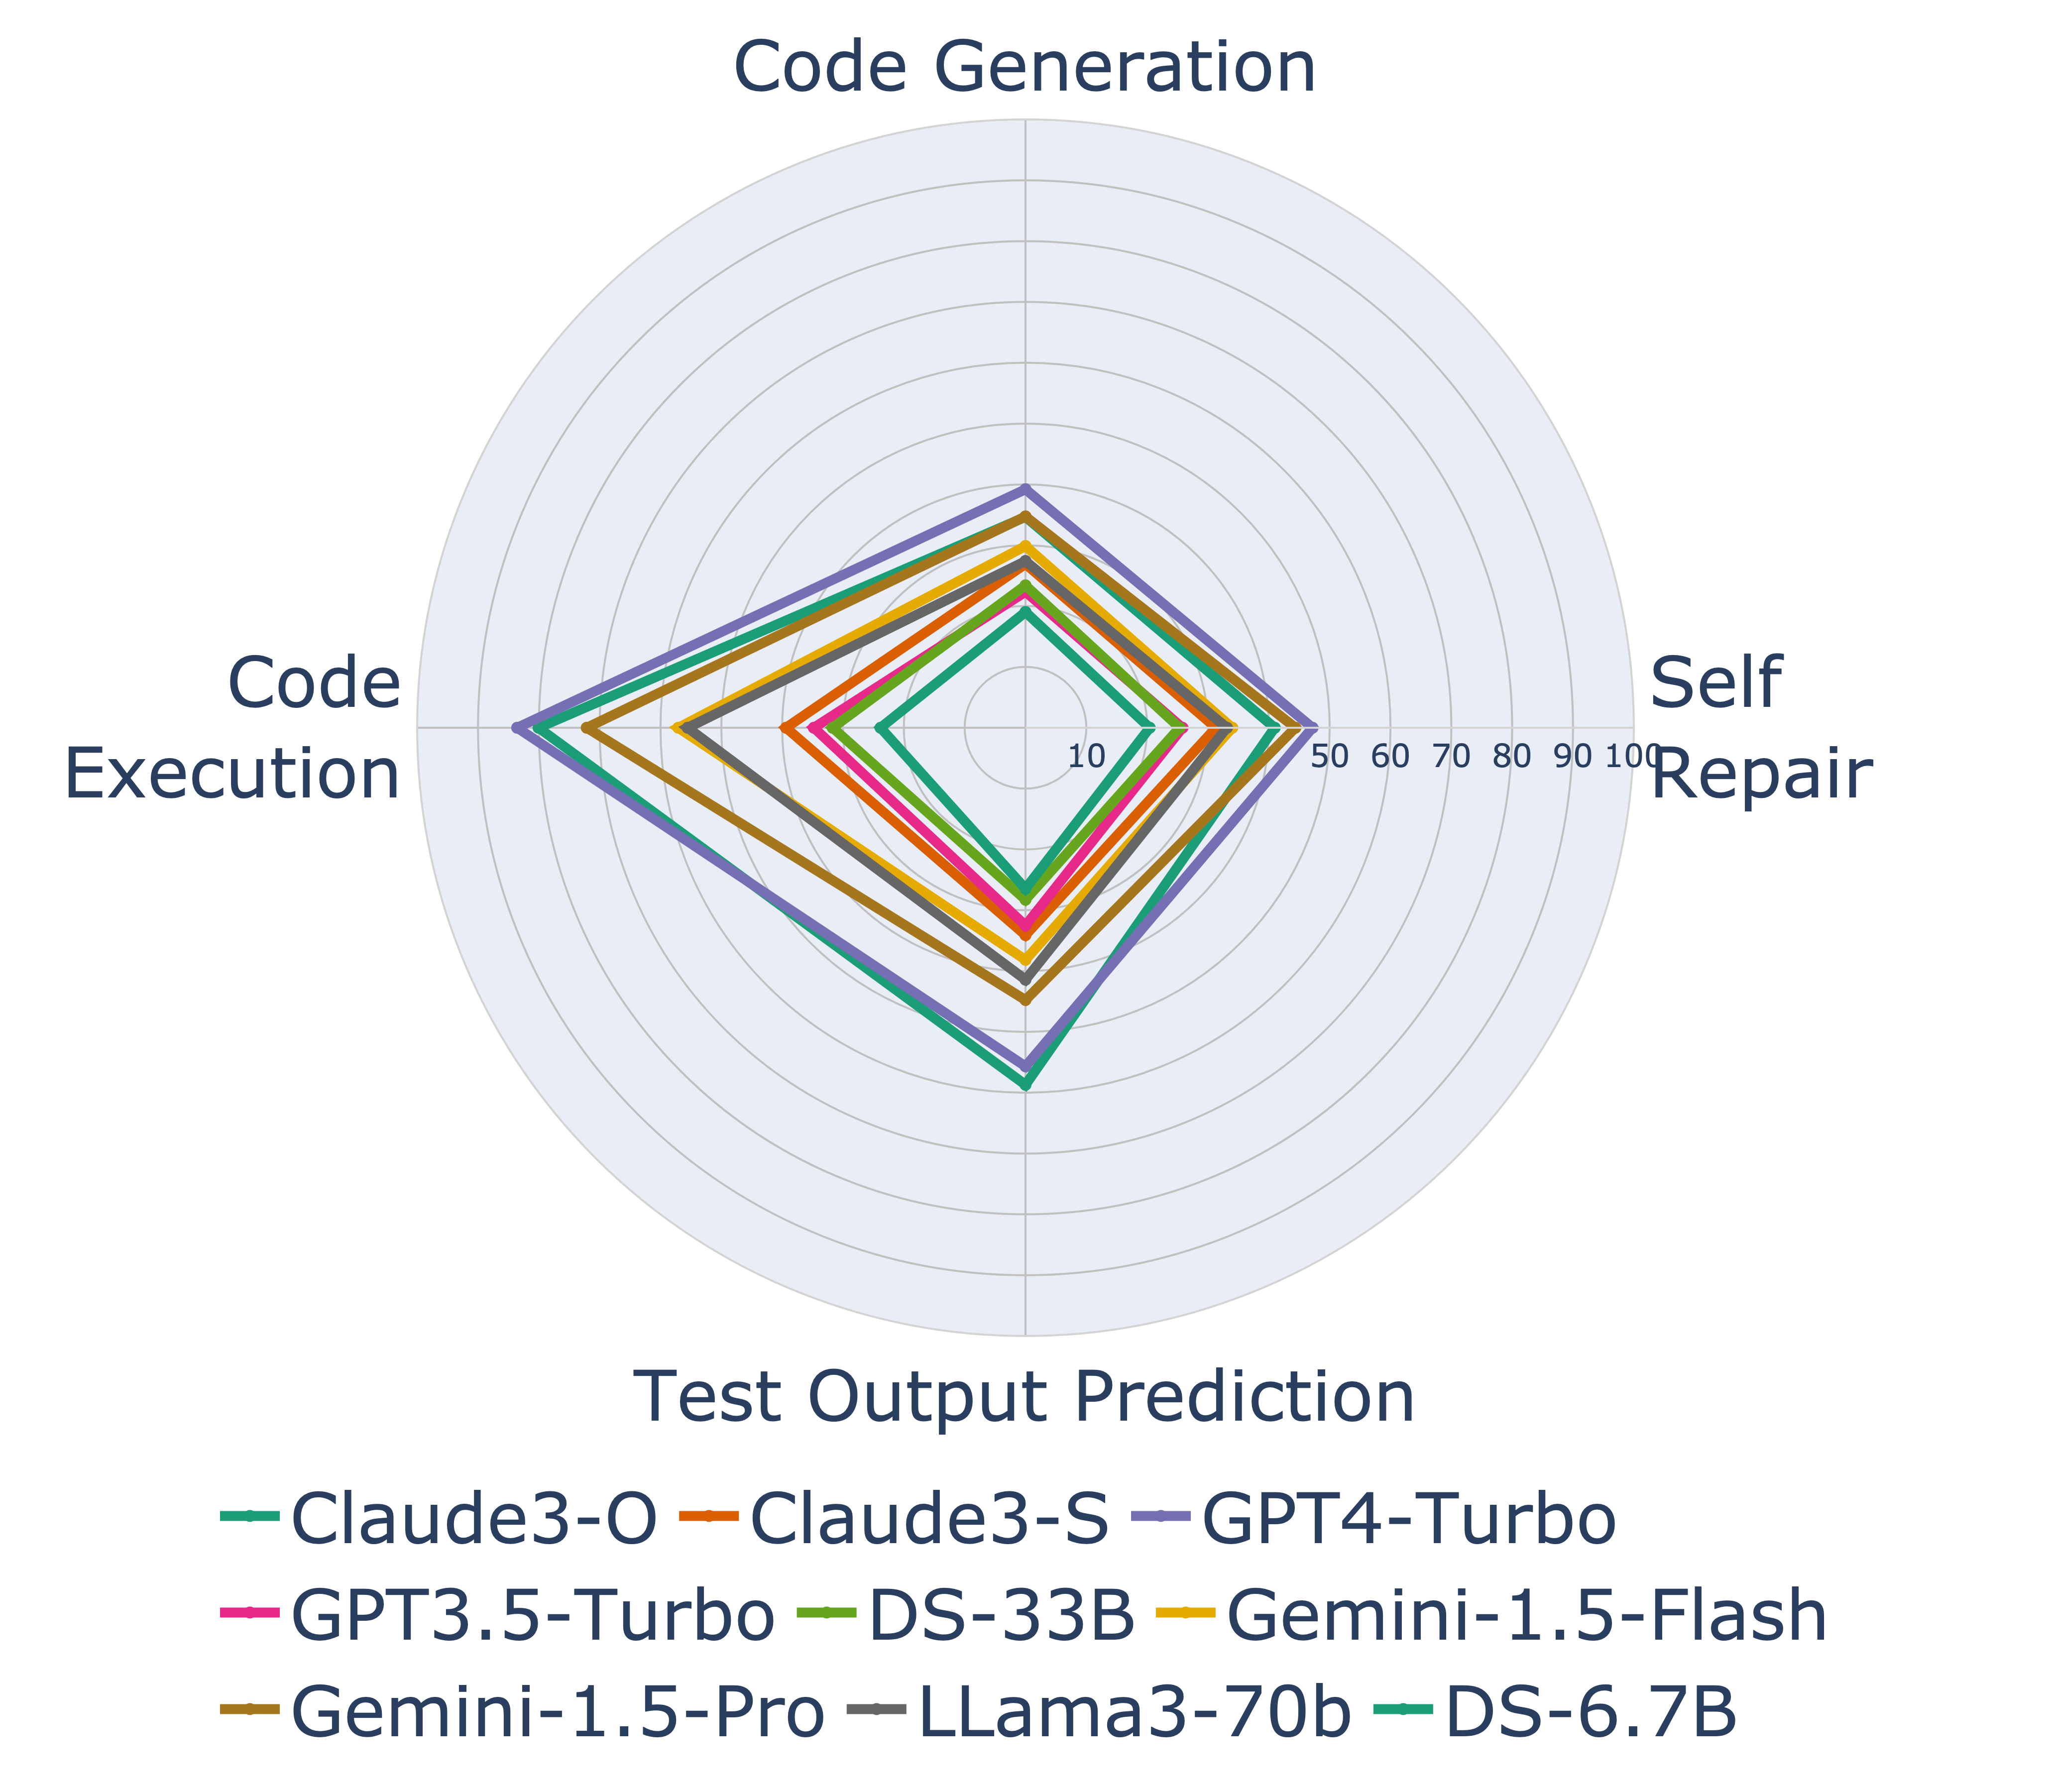
\includegraphics[width=0.435\linewidth]{figures/overview/tasks_radar.png}

        \vspace{-3pt}

    % 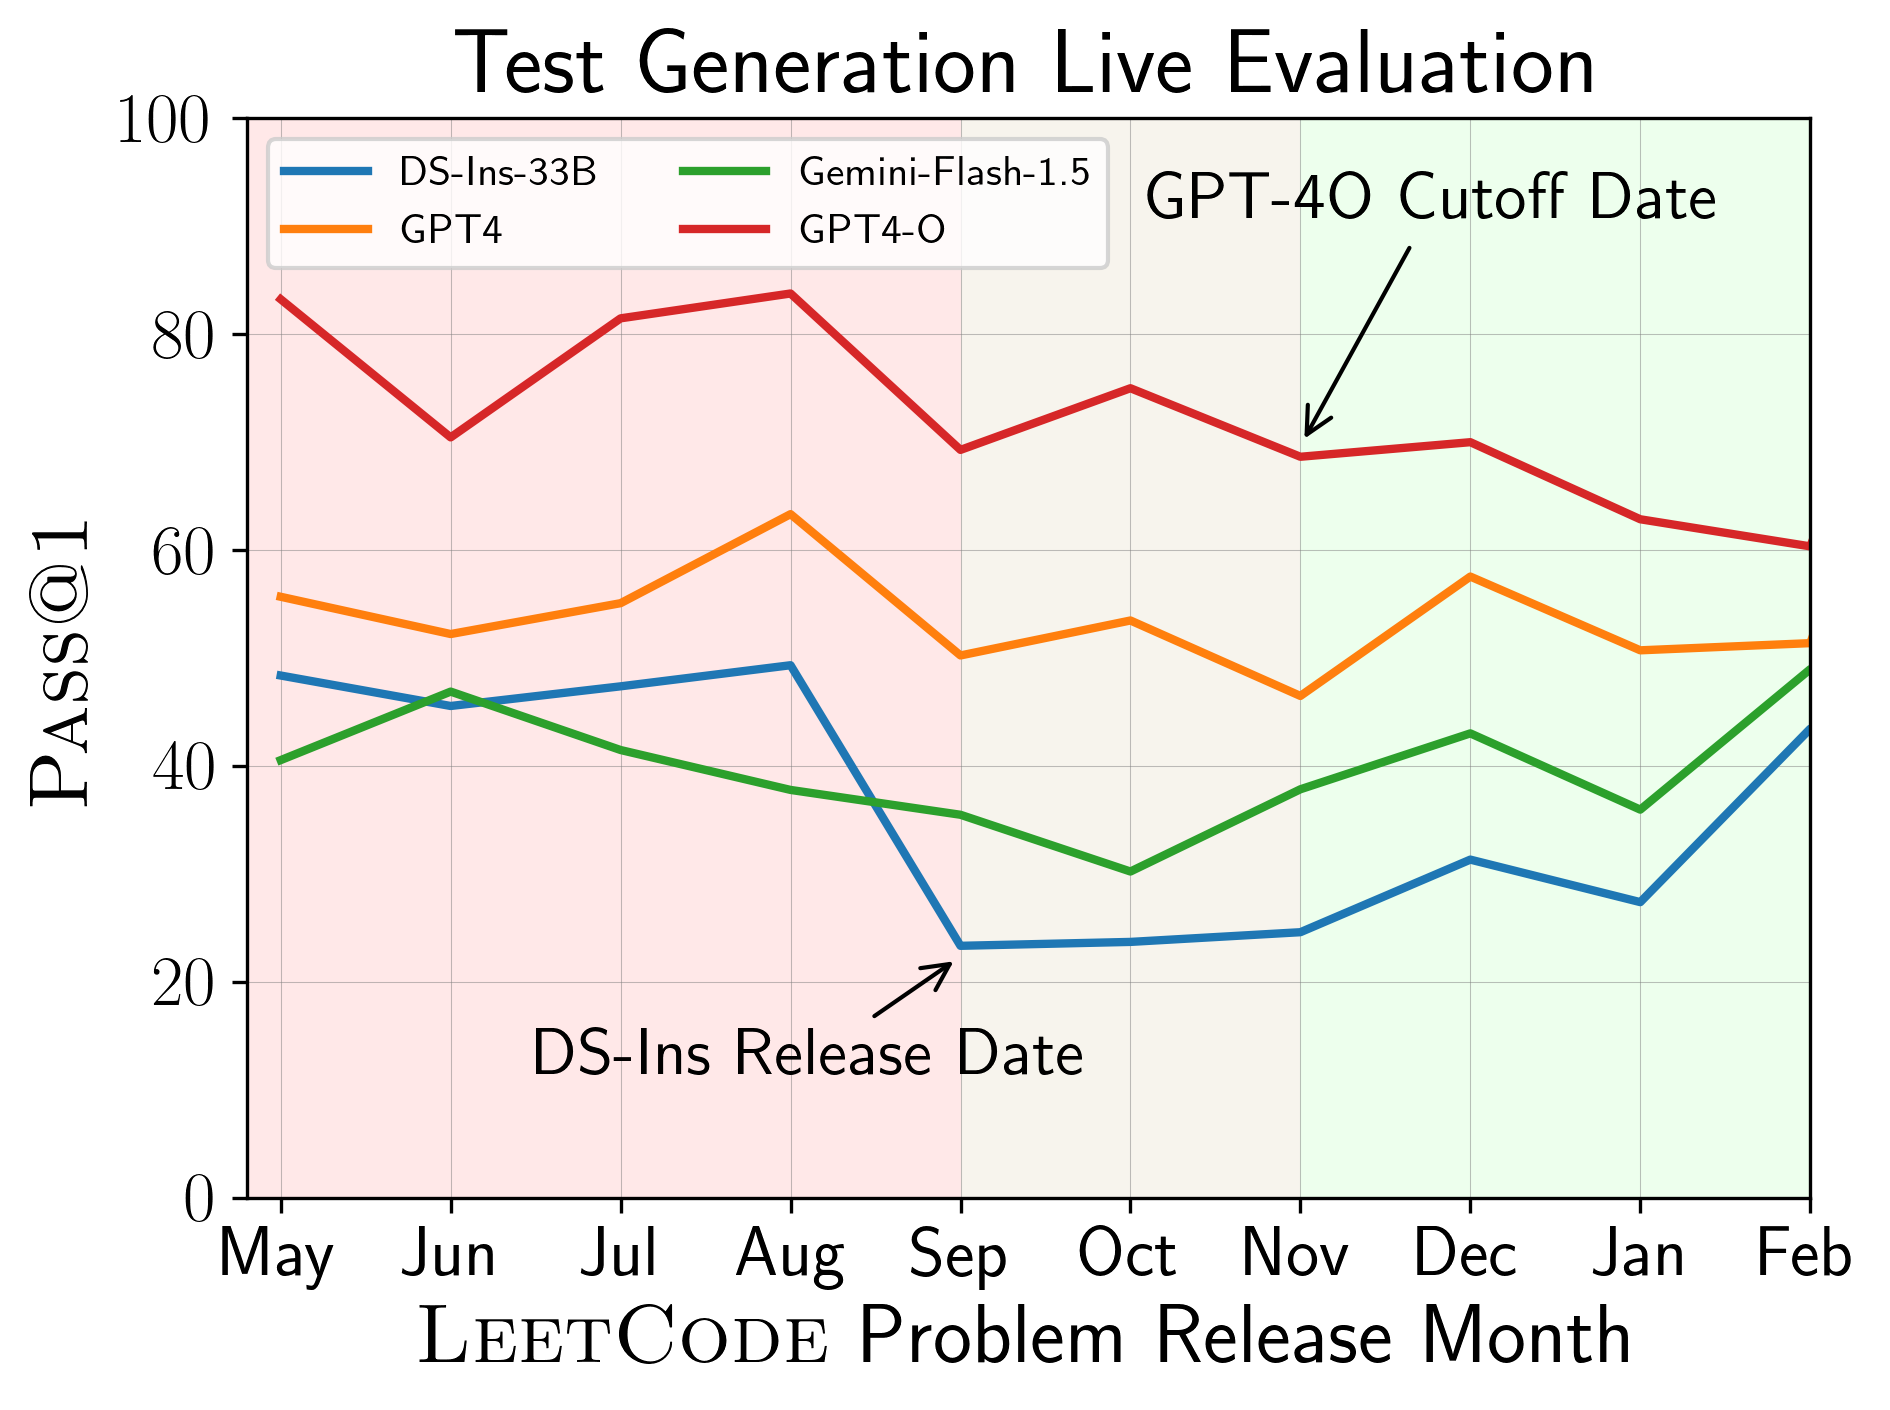
\includegraphics[width=0.49\linewidth]{figures/contamination_new/main_14_testgen_leetcode.png}%
    \caption{
        \textbf{Left.} \livecodebench{} comprises problems marked with release dates, allowing evaluations over different time windows.
        The figure depicts performances of \deepseek{}, \gptfouro{}, and \claudethrees{} models over bimonthly time windows ($\sim40$ \leetcode{} problems) showcasing a stark drop after their cutoff dates, highlighting contamination.
        Thus, we can detect and avoid contamination by evaluating models only on time-windows after the model's cutoff date (green region)\protect\footnotemark.
          \textbf{Right.} We evaluate \llms{} across 
        four scenarios that capture key coding capabilities necessary for building programming agents: code generation, repair, testing, and comprehension.
        %Specifically, we host four different scenarios, namely code generation, 
        %self-repair, code execution, and test output prediction.
        The figure depicts various model performances across the scenarios available in \livecodebench{} in a radial plot -- 
        highlighting relative differences changing across the scenarios.
        }
    \label{fig:contamination_main}
    \vspace{-10pt}
\end{figure}

\footnotetext{Note that for model comparisons -- performances are averaged across multiple months and platforms achieving a larger sample size.}